\chapter{Standardize Graph Data}
\label{Ch-2:Sec:Standardize}

In this part, we'll extract the wiki data from the public wiki API and design the graph structure from it.\\
For the original raw data, we choose the semi-structure data from \href{http://www.tolkiengateway.net}{Tolkien Gateway Website}\footnote{http://www.tolkiengateway.net} also known as TG. This is a not-for-profit collaborative wiki which aims to collect and organize the works of J.R.R. Tolkien for fans and researchers, like a Tolkien encyclopedia, while Tolkien Estate holds the copyright over the literary texts\footnote{https://en.wikipedia.org/wiki/Tolkien\_Estate}. What's more, Tolkien Gateway has become the largest and most well-built Tolkien-related encyclopedia on the World Wide Web since 2010 based on \href{http://tolkiengateway.net/wiki/List\_of\_Tolkien\_Encyclopedias}{research} by Mith\footnote{Noticing that \href{https://lotro-wiki.com/}{LOTRO-Wiki} on the top of the list with \href{https://lotro-wiki.com/index.php/Special:Statistics}{86,649 articles} is a game wiki exclusively ``\href{https://lotro-wiki.com/index.php/Lord_of_the_Rings_Online}{Lord of the Rings Online}''-related. Thus, it isn't a good choice to do the research work based on a Massively Multiplayer Online Role-Playing Game set in Tolkien's Middle-Earth.}, which gives \footnote{\href{https://lotro-wiki.com/index.php/Lord\_of\_the\_Rings\_Online}{LOTRO-Wiki}, ``\href{https://lotro-wiki.com/index.php/Special:Statistics}{Statistics}'' (retrieved 15 March 2019)}. It offers \href{http://tolkiengateway.net/w/api.php}{APIs}\footnote{Tolkien Gateway, ``\href{http://tolkiengateway.net/w/api.php}{API}'' (retrieved 15 March 2019)} with documents in detail for users to craw data from its website. The APIs are a little bit different from the ones of Wikipedia, so we'll discuss them in the following subsections.

\section{Problem Statement}
\label{Ch-2:Sec:Problem Statement}

From this subsection, we begin to state our problem definition. The data structure from Tolkien Gateway is like the one from Wikipedia. Raw data shared by \href{http://www.gnu.org/licenses/fdl-1.3.en.html}{GNU Free Documentation License}\footnote{\href{http://www.gnu.org/licenses/fdl-1.3.en.html}{http://www.gnu.org/licenses/fdl-1.3.en.html}} which we can get directly from request messages by using web crawlers through TG APIs and save the data into local text files for the next steps. Then, based on the paper of \cite{zesch2007analysis}, an article graph and a category graph can be set up from the raw data. 
As this search engine needs to meet the requirements of Graph discovery and natural language process, an undirected graph with labels and attributes is necessary to the experiment, which can also fit the structure of wiki pages (articles) with categories. \\
So, we define the input raw data as $D := (P, C)$, and the output graph as $G := (V, L, A, E)$. $D$ represents raw data combined with $P$ as wiki article/content pages and $C$ as category pages. $G$ refers to the undirected Graph we need to build from $D$ to store these relationships, including $V$ as vertices, a collection of nodes (article Ids); $L$ as labels, a collection of nodes (category Ids), separated with $V$ by different shapes and colors; $A$ as attributes (option), a small set of nodes with attribute names described one article vertex $v \in V$ detailedly; $E$ as edges, a group of relationships between nodes (four different kinds: $V$ and $V$, $L$ and $L$, $V$ and $L$, $V$ and $A$) (\cite{newman2003structure}). 

\section{Related Work}
(unfinished)

\label{Ch-2:Sec:Related Work}
\cite{zesch2007analysis}, taxonomy-like structure WCG and article graph
\cite{bibid}

\section{Summary of Technique}
\label{Ch-2:Sec:Summary of Technique}

To get the raw data from a wiki farm, clean the data and change the semi-structure files into a graph, we use these technique listed below.

\subsection{Web Crawler Frame with Scrapy}

\href{https://scrapy.org/}{Scrapy}\footnote{https://en.wikipedia.org/wiki/Scrapy} is an open-source web-crawling framework which works with Python program using \href{http://www.linfo.org/bsdlicense.html}{BSD License}\footnote{https://en.wikipedia.org/wiki/BSD\_licenses}. It can be used as a data extraction with APIs or as a general-purpose web crawler\footnote{\href{https://scrapy.org/}{https://scrapy.org/}}. This framework can help us to get raw data from a wiki farm. The raw data can be set in many structures. Considering the convenience for next steps, the data is organized in Extensible Markup Language (XML). Scrapy also offers a demo frame which can help users build their own crawler.\\

\subsection{Extract Data with Scrapy Selectors}
Next, we need to extract data from the XML sources. \href{https://www.crummy.com/software/BeautifulSoup/}{BeautifulSoup} is a popular web scraping python library though a little bit slow\footnote{\href{https://www.crummy.com/software/BeautifulSoup/}{https://www.crummy.com/software/BeautifulSoup/}} and \href{http://lxml.de/}{lxml} is a XML parsing library with ElementTree API\footnote{\href{http://lxml.de/}{http://lxml.de/}} though not in Python standard library. Thus, we choose to use Scrapy Selectors for data extraction. Categories (id, name), category tree and articles (id, name, detail, inner link) can be stored after this step.

\subsection{Output Category and Article Graph with igraph}
Finally, we need a library to build an undirected graph with labels and attributes. igraph is an open source package with network analysis tools, well-known for its high efficiency and portability, supporting R, Python, Mathematica and C/C++.

\section{Implementation}
We use Scrapy demo frame to build three major crawlers to get the categories, articles and inner links betweens them. In \nameref{fig:section2-pic1}, the processes are explained in detail listed below.

\begin{figure}
	\centering
	\def\svgwidth{\columnwidth}
	\input{fig/Section2.pdf_tex}
	\caption{Process of Standardizing Graph Data}
	\label{fig:section2-pic1}
\end{figure}

\subsection{URL Crawler}

This crawler is labeled as jrrtgateway\_url\_scrapy in \nameref{fig:section2-pic1}.

\begin{enumerate}
	\item Focus three category roots (``Eä'', ``Real-world'' and ``Other fictional worlds'') in this wiki. Take ``Eä'' as example. Set API parameters as {action: ``query'', list: ``categorymembers'', cmlimit: 1000, format: ``xml'', cmtitle: ``Category:Eä''}. Put ``Eä'', ``Real-world'' and ``Other fictional worlds'' in stack $S$ and dictionary $L$.
	\item Pop the last item $i$ in the stack, change ``cmtitle'' to ``Category:$i$'' and run the crawler. 
	\item Extract data from XML files returned by API request and get children's ids and names (including categories, articles, files and other special pages). If a child is still a category, push the category name into the stack $S$, add category id to the key of $L$ and set category name as value. If a child is an article, add article id to the key of $V$ and set article name as value. Then, append the relationships between $l$ and $l$ or $l$ and $v$ to list $E$.
	\item Repeat step 2 and 3, until stack $S$ is empty.
\end{enumerate}

\subsection{Article Crawler}

This crawler is labeled as jrrtgateway\_article\_scrapy in \nameref{fig:section2-pic1}.

\begin{enumerate}
	\item Get article Ids $K$ from $V$ keys.
	\item Set API parameters as {action: ``query'', prop: ``revisions'', rvprop: ``content'', format: ``xml'', pageids: ``$k$''} and run the crawler. 
	\item Clean the detailed data and extract attributes $a$ for each article.
	\item Repeat Step 2 and 3, until get all article details and attributes.
\end{enumerate}

\subsection{Inner Links Crawler}

This crawler is labeled as jrrtgateway\_inner\_scrapy in \nameref{fig:section2-pic1}.

\begin{enumerate}
	\item Get article Ids $K$ from $V$ keys.
	\item Set API parameters as {action: ``query'', generator: ``links'', gpllimit: ``max'', format: ``xml'', pageids: ``$k$''} and run the crawler. 
	\item Extract inner link nodes and add the relationships between vertices to edges $E$.
	\item Repeat Step 2 and 3, until get all article inner links.
\end{enumerate}

Finally, merge the clean data extracted from the results of three crawlers shown in \nameref{fig:section2-pic234}.

\begin{figure}
	\centering
	\begin{subfigure}{0.31\textwidth}
		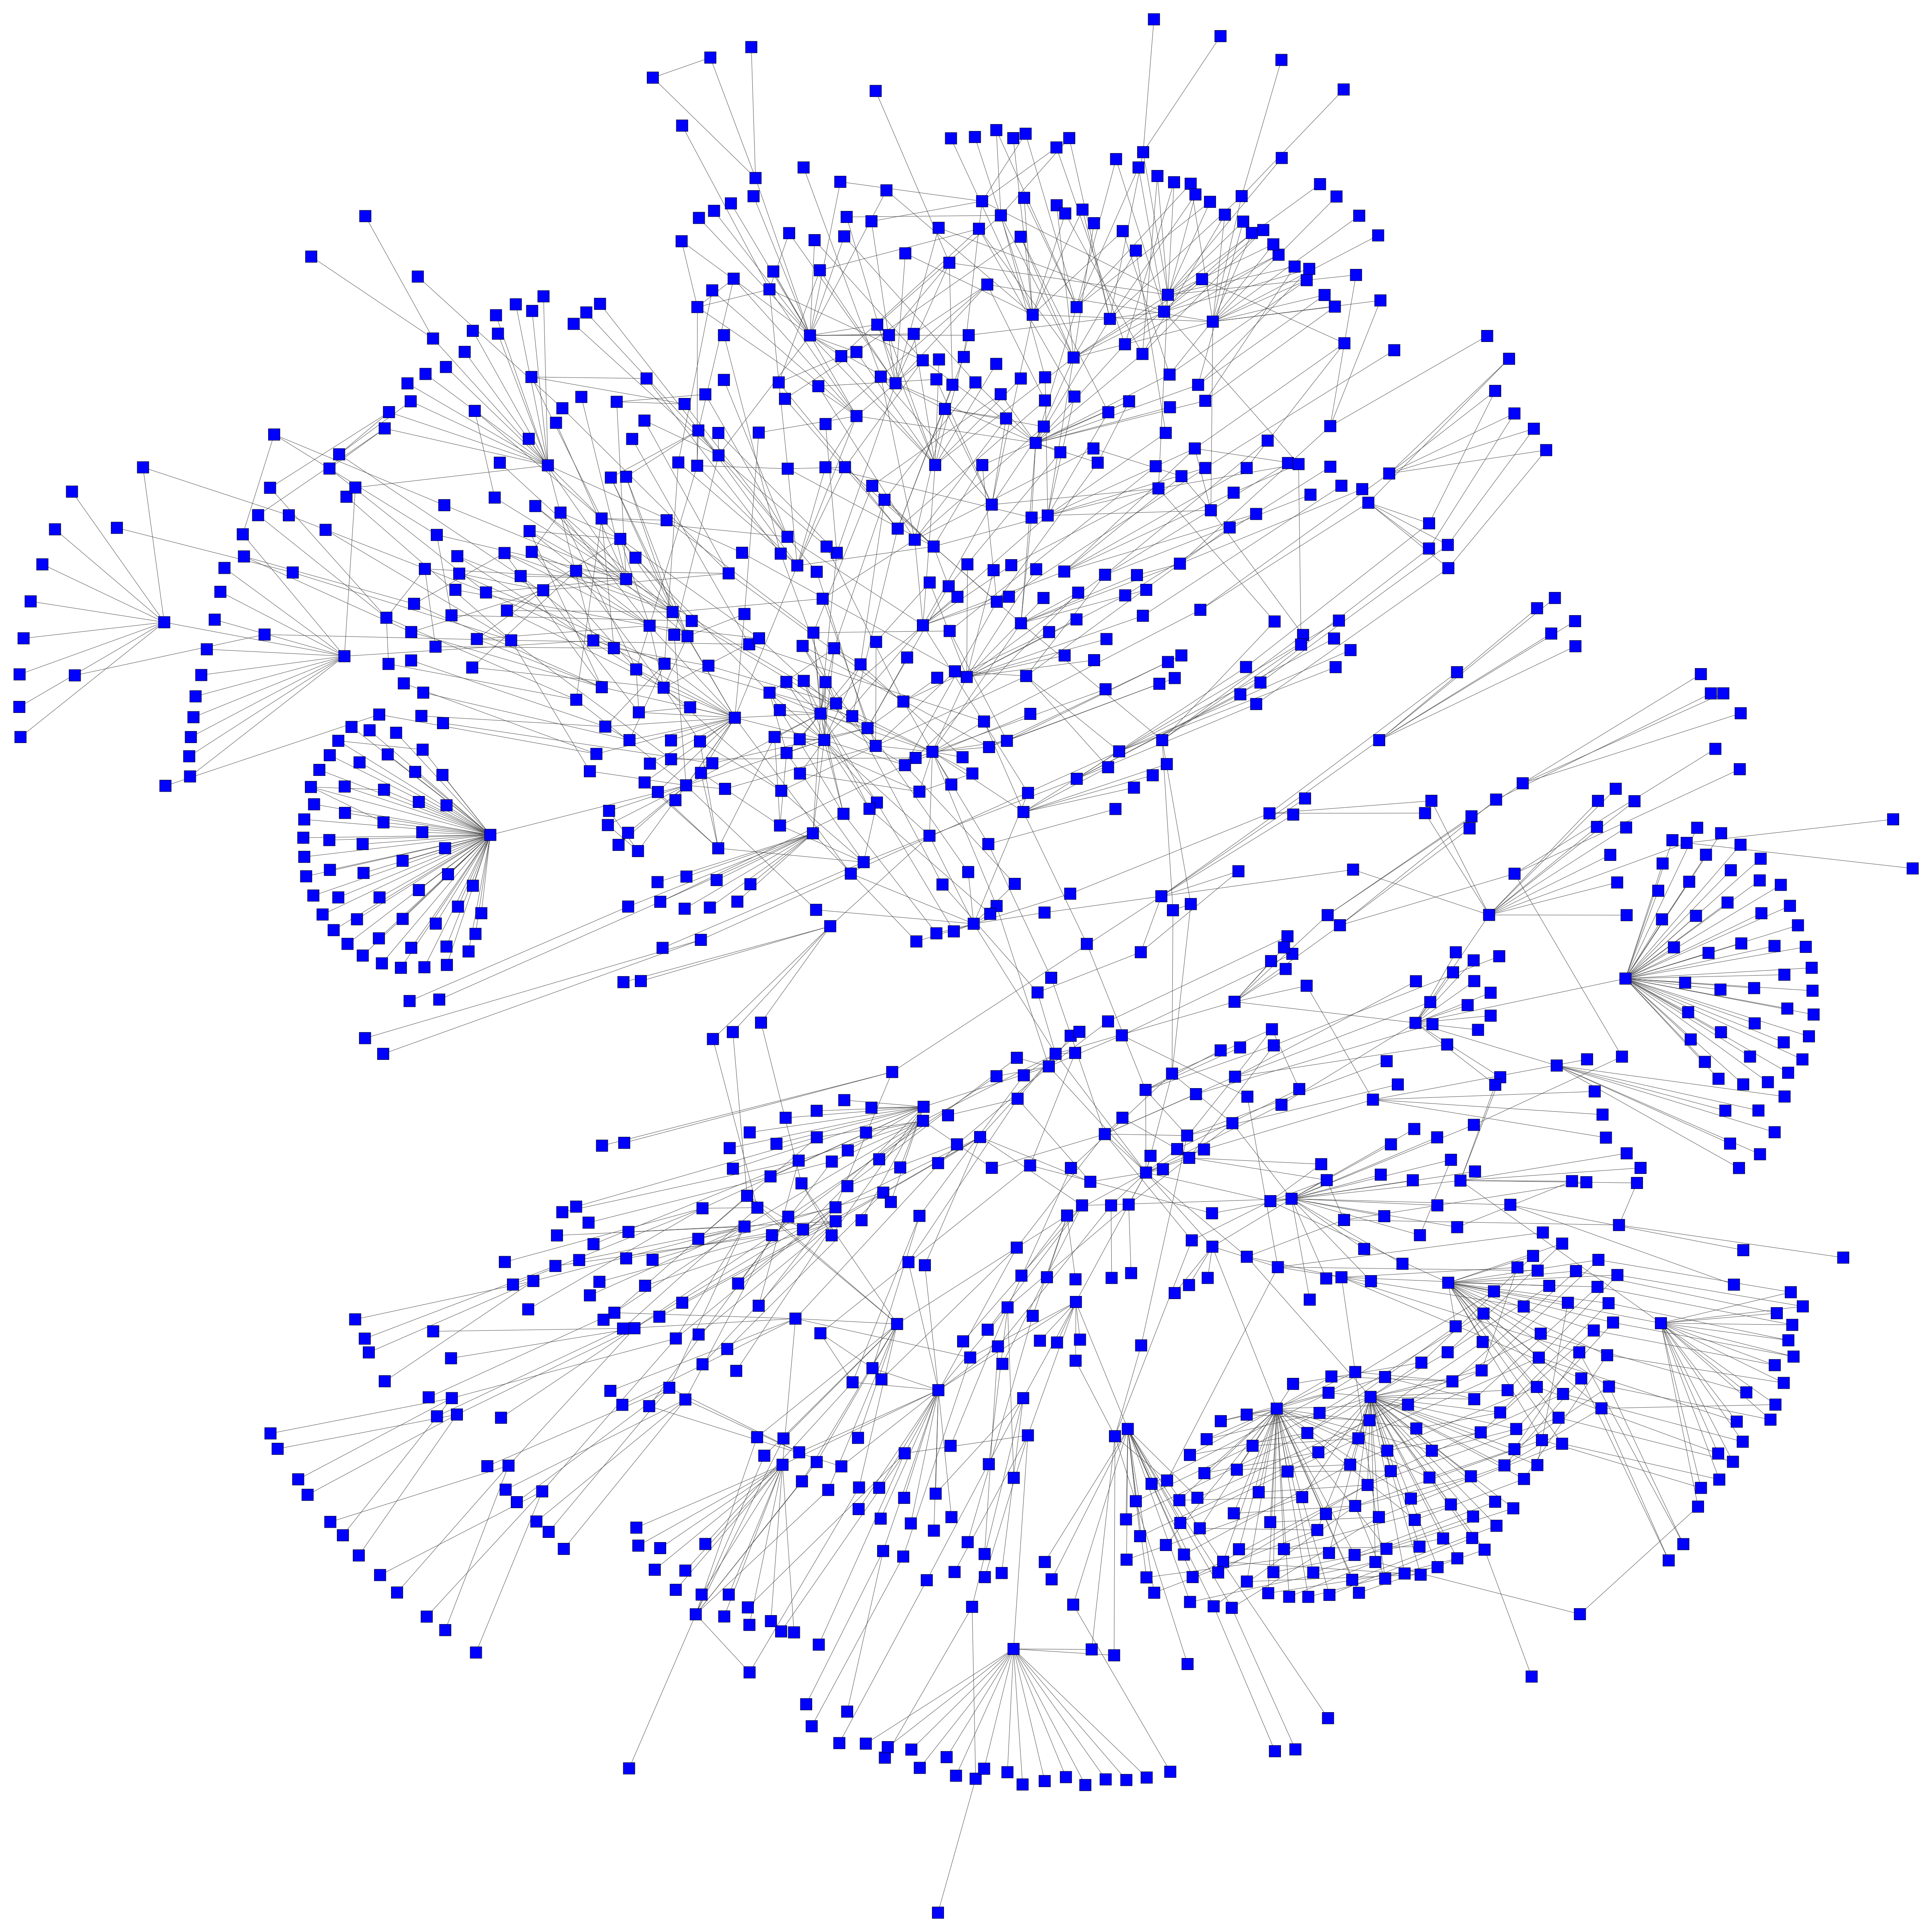
\includegraphics[width=\linewidth]{fig/graphs_category_c.png}
		\caption{Category Graph} 
		\label{fig:section2-pic2}
	\end{subfigure}
	\hspace*{\fill} % separation between the subfigures
	\begin{subfigure}{0.31\textwidth}
		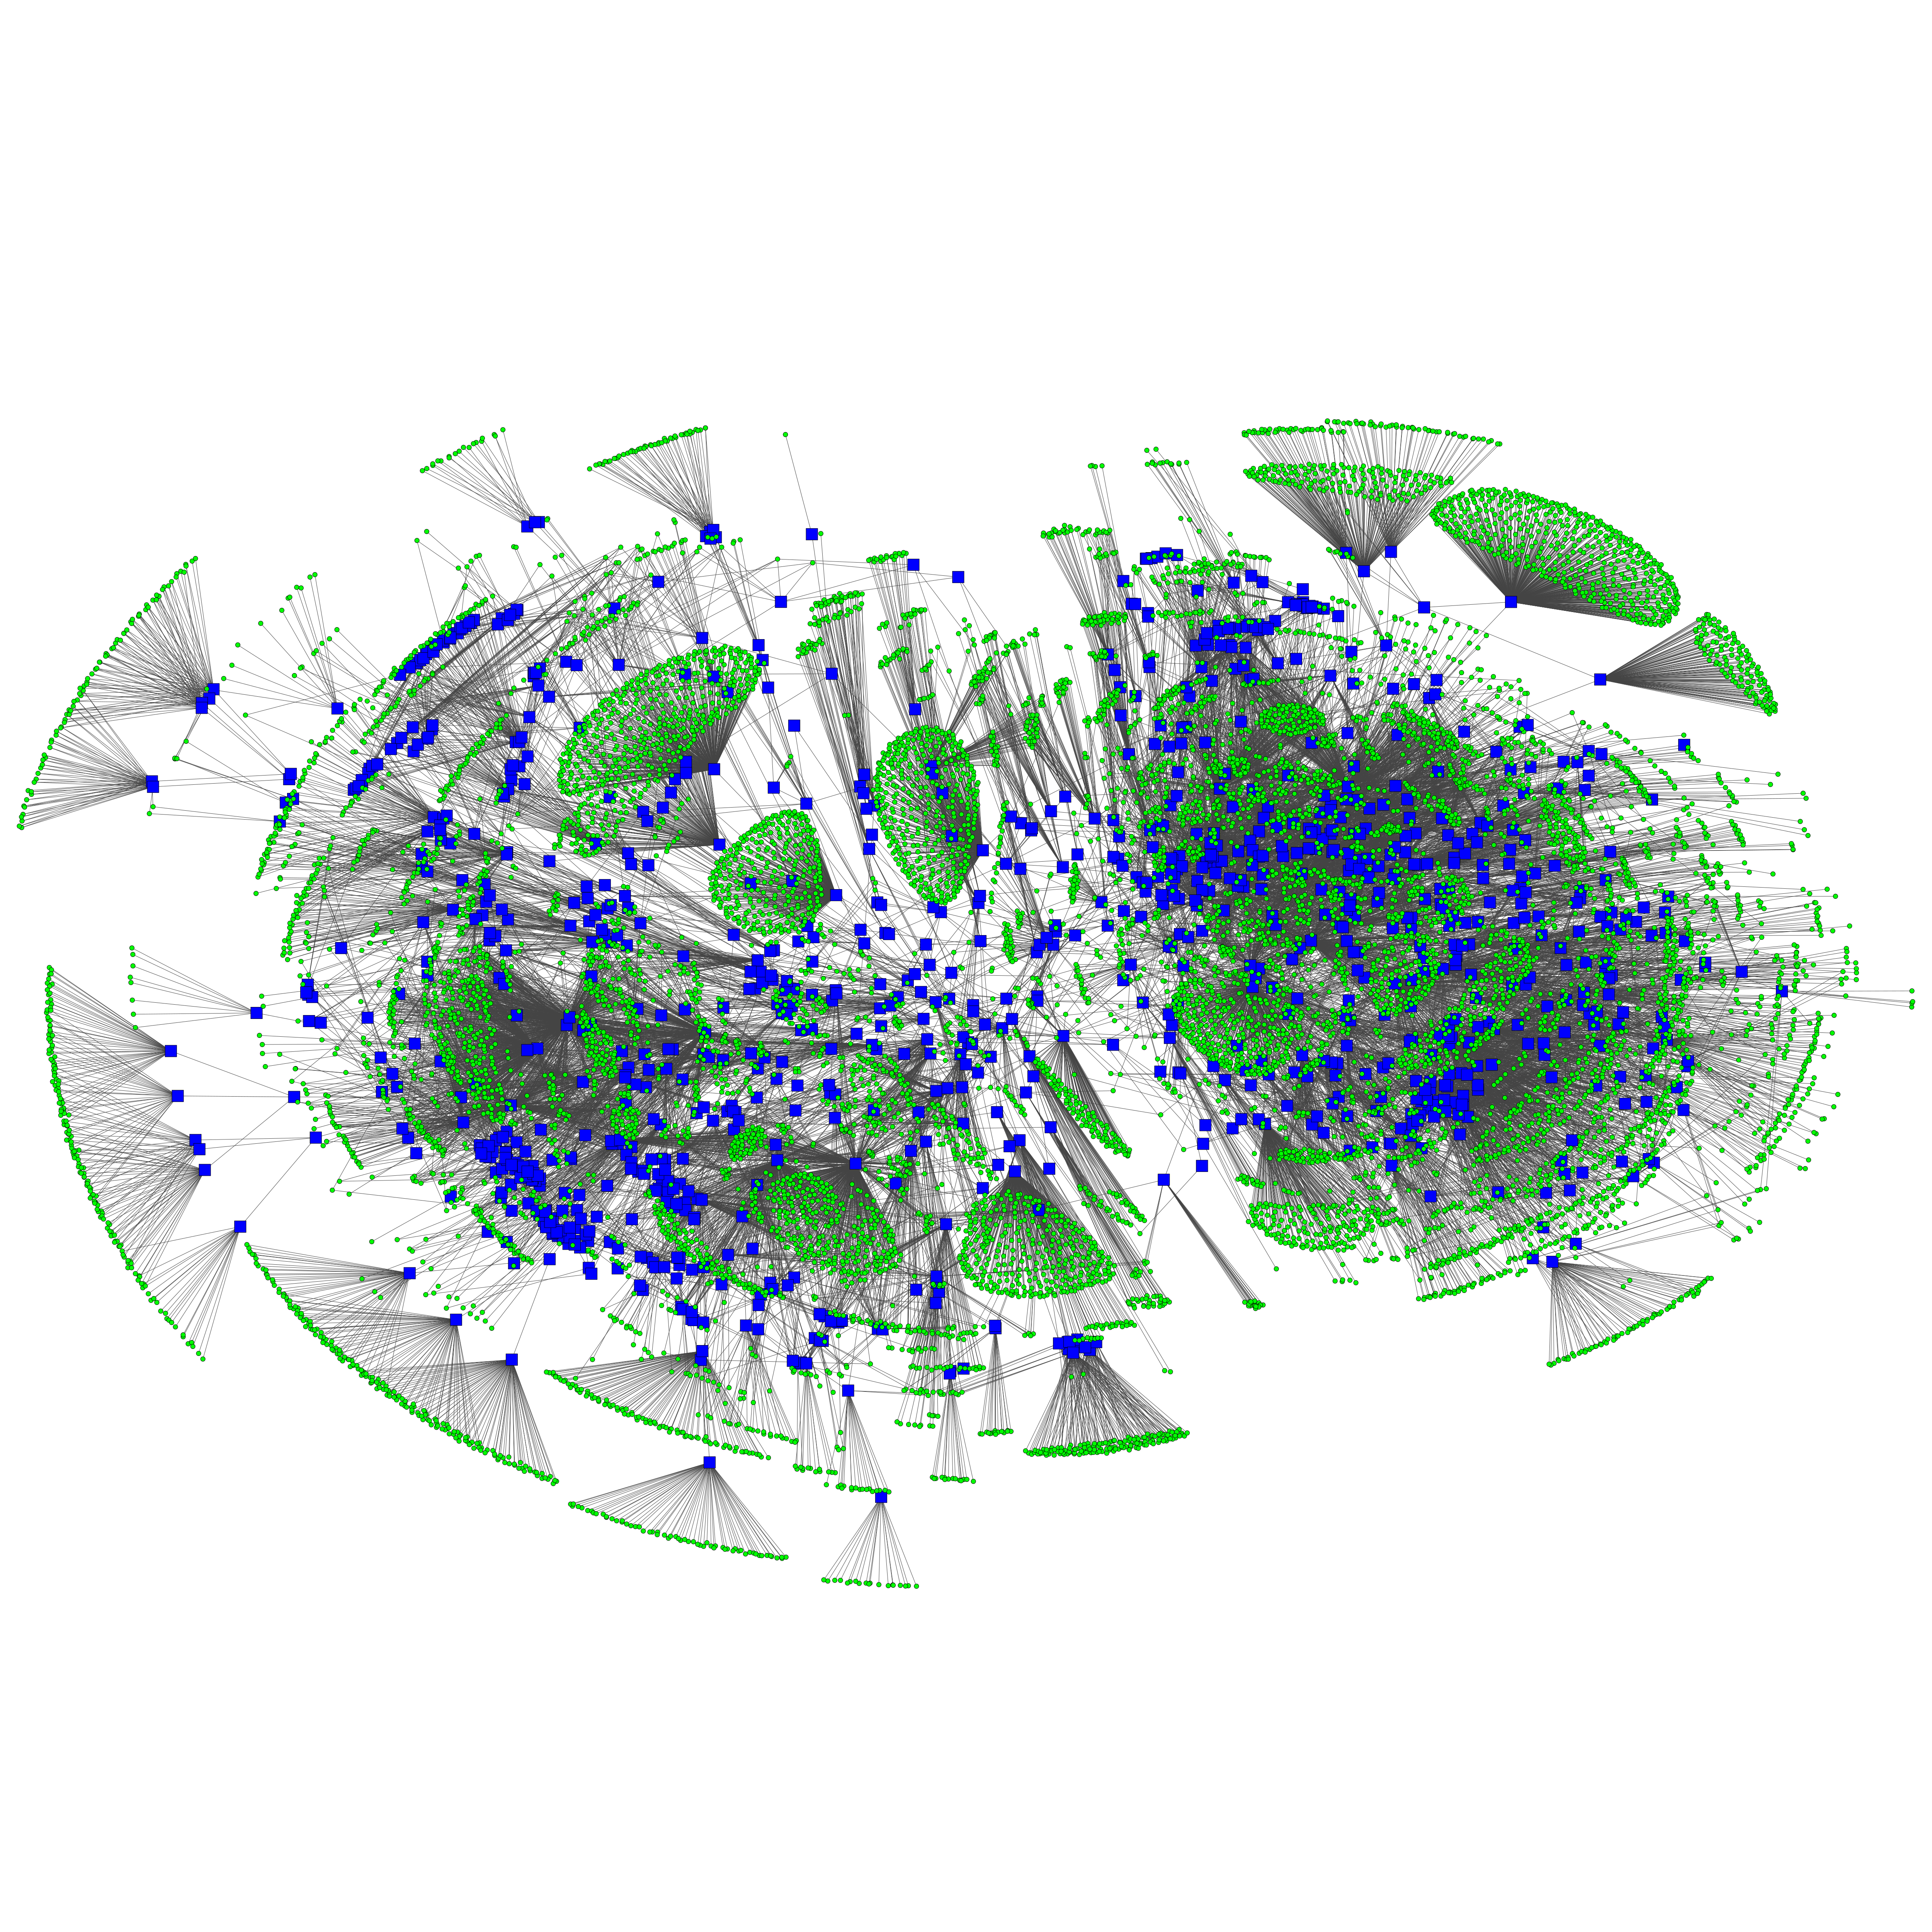
\includegraphics[width=\linewidth]{fig/graphs_category_ca.png}
		\caption{Article with Category} \label{fig:section2-pic3}
	\end{subfigure}
	\hspace*{\fill} % separation between the subfigures
	\begin{subfigure}{0.31\textwidth}
		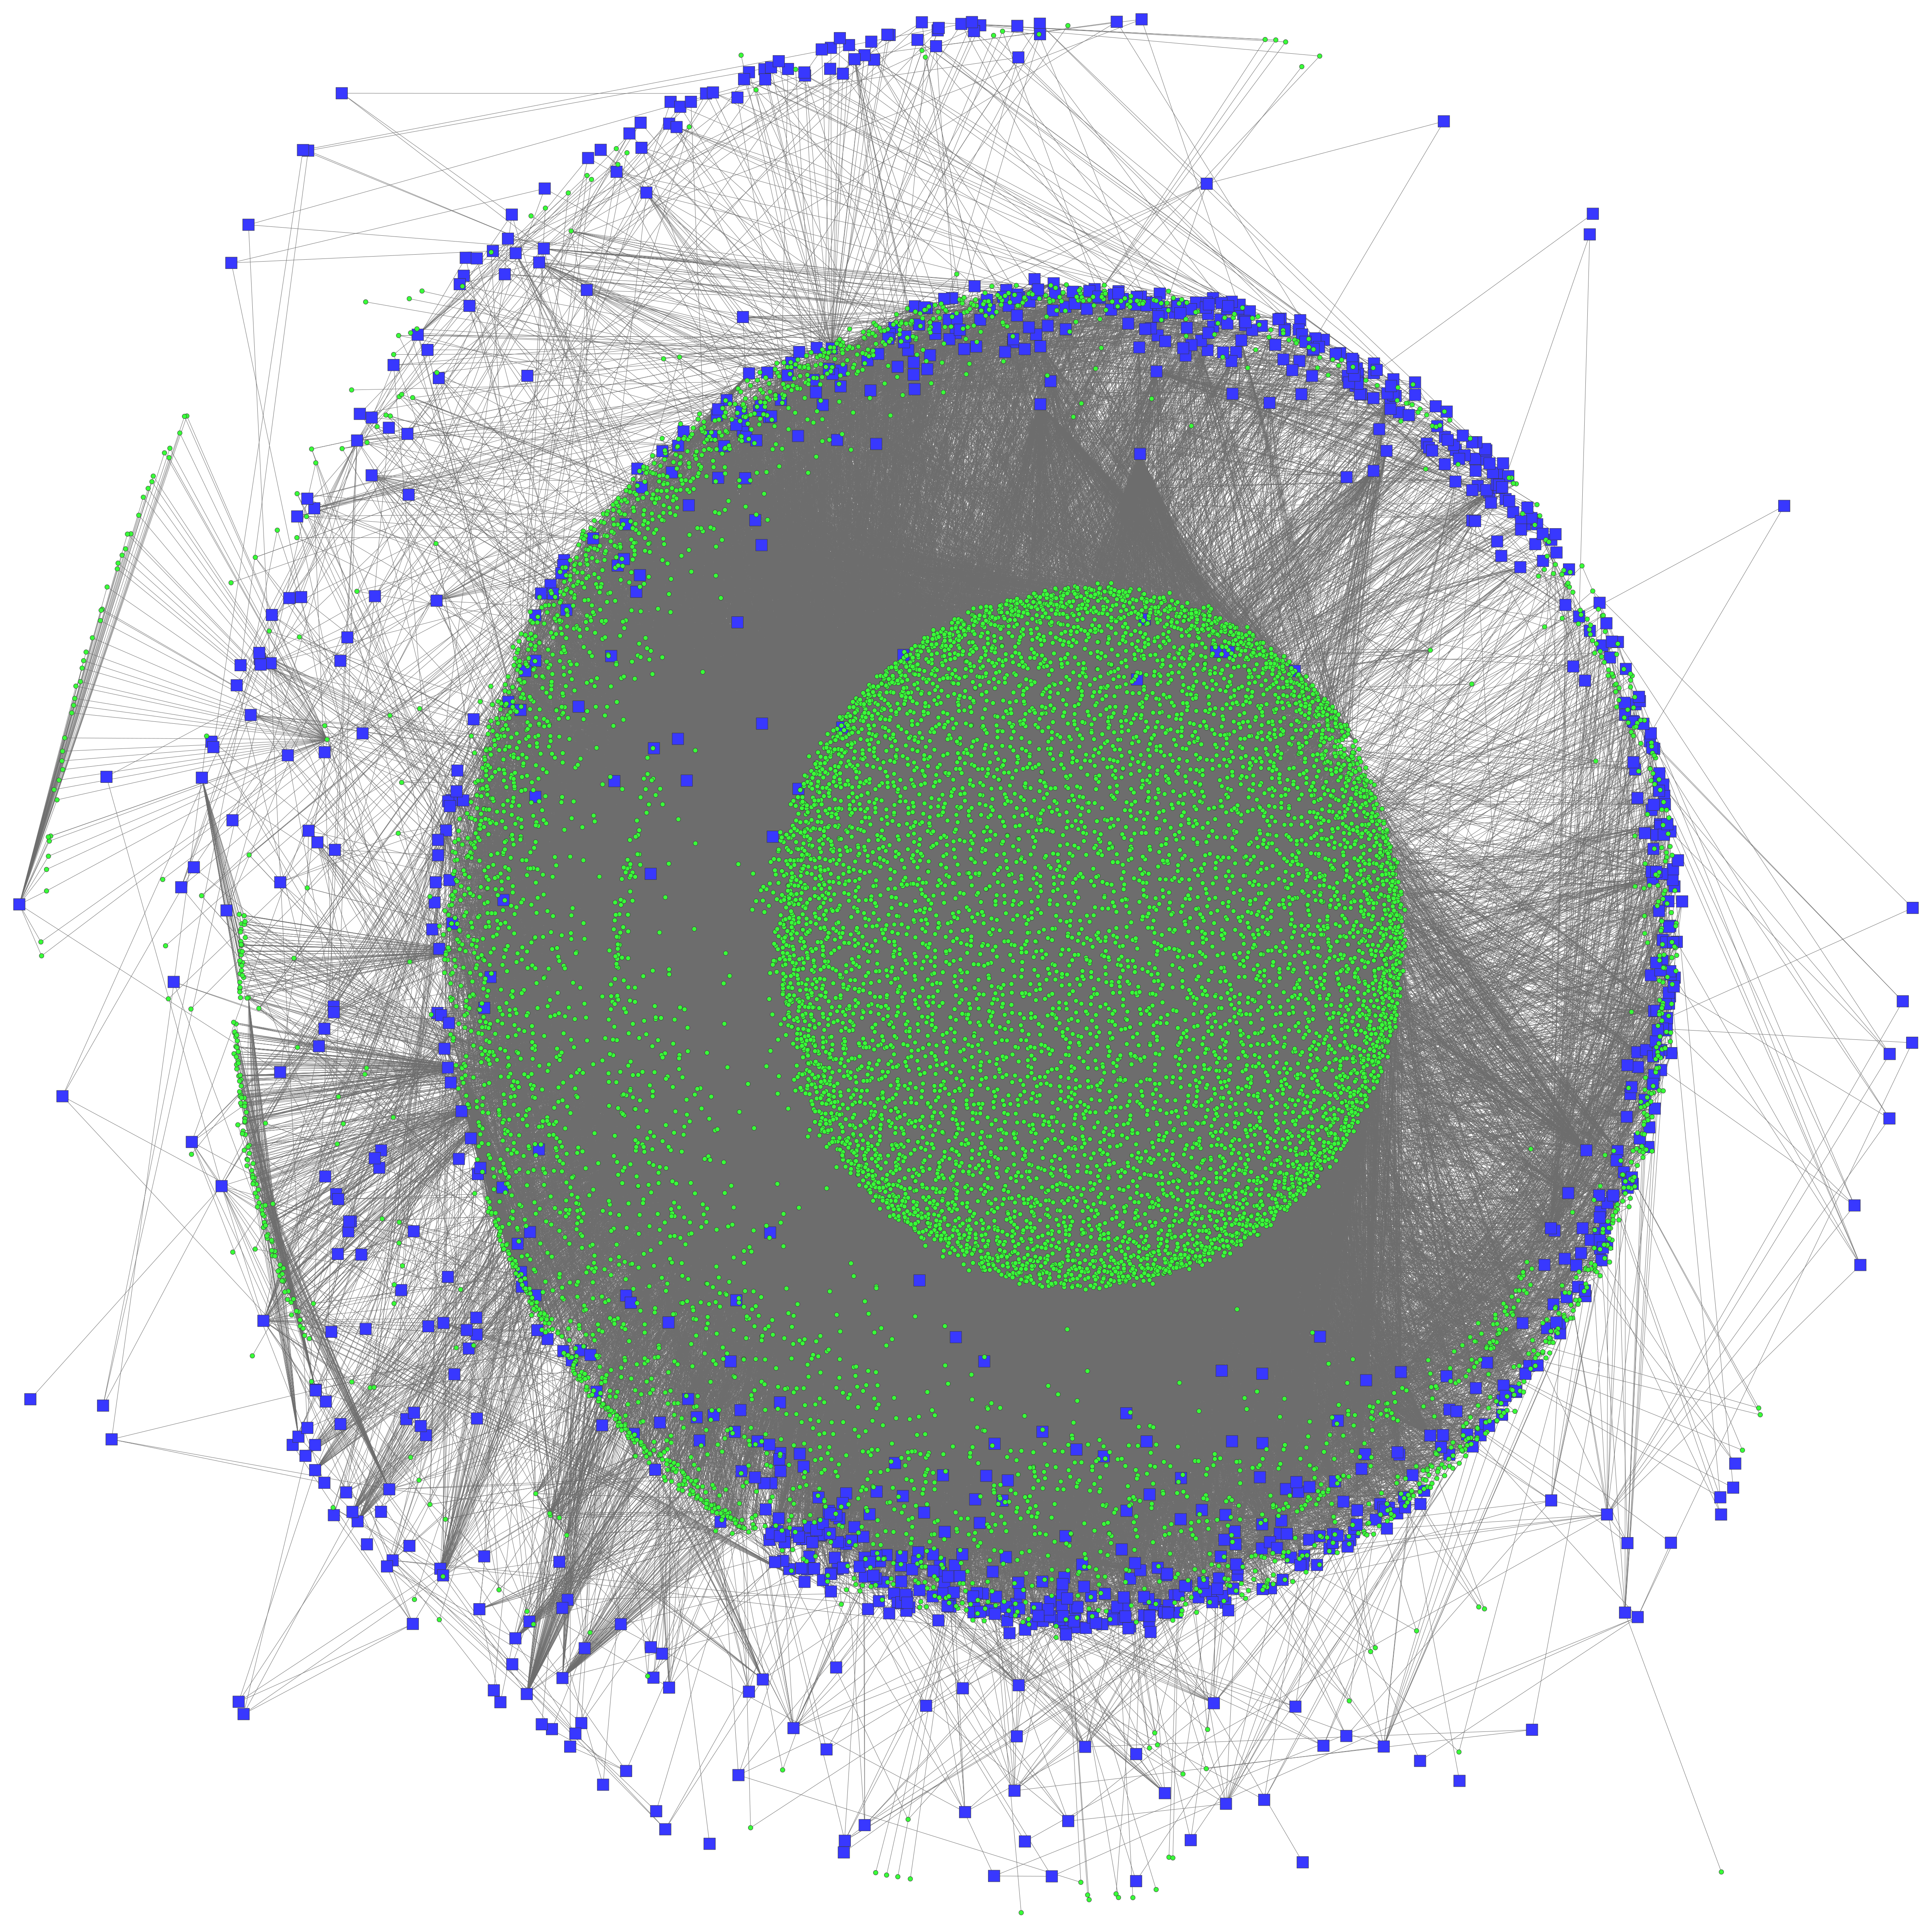
\includegraphics[width=\linewidth]{fig/graphs_category_a.png}
		\caption{Category-Article Graph} \label{fig:section2-pic4}
	\end{subfigure}
	\caption{Process of Standardizing a Graph from Raw Data} \label{fig:section2-pic234}
\end{figure}

\section{Conclusion}
(unfinished)



